\documentclass[convert={density=300,size=1080x800,outext=.png}]{standalone}
\usepackage{tkz-graph}
\usetikzlibrary{arrows,positioning,shapes,shapes.multipart,patterns,mindmap,shadows}
\usepackage{xcolor}
\usepackage{helvet}
\renewcommand{\familydefault}{\sfdefault}


\begin{document}

\footnotesize
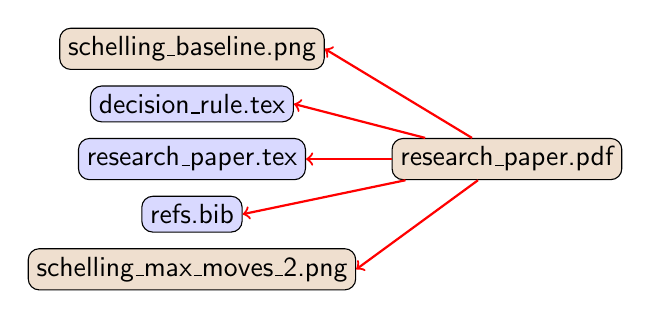
\begin{tikzpicture}[every node/.style={
    rectangle,
    rounded corners,
    inner sep=3pt,
    draw,
    fill=brown!25
}]
    \node (schelling_baseline_png) [shift={(5, 1.4)}]
    {
        schelling\_baseline.png
    };
    \node (decision_rule_tex) [fill=blue!15, shift={(5, 0.7)}]
    {
        decision\_rule.tex
    };
    \node (schelling_max_moves_2_png) [shift={(5, -1.4)}]
    {
        schelling\_max\_moves\_2.png
    };
    \node (refs_bib) [fill=blue!15, shift={(5, -0.7)}]
    {
        refs.bib
    };
    \node (research_paper_tex) [fill=blue!15, shift={(5, 0)}]
    {
        research\_paper.tex
    };
    \node (research_paper_pdf) [shift={(9, 0)}]
    {
        research\_paper.pdf
    };
    \draw[->, red, thick] (research_paper_pdf) to (schelling_baseline_png.east);
    \draw[->, red, thick] (research_paper_pdf) to (decision_rule_tex.east);
    \draw[->, red, thick] (research_paper_pdf) to (research_paper_tex);
    \draw[->, red, thick] (research_paper_pdf) to (refs_bib.east);
    \draw[->, red, thick] (research_paper_pdf) to (schelling_max_moves_2_png.east);
\end{tikzpicture}

\end{document}